\documentclass[pdf]{beamer}
\newcommand\REV{v0.0.1}
% Berlin Berkeley Warsaw
\newcommand\z[1]{\texttt{#1}}
\usepackage{listings}
\usepackage{xeCJK}
\newcommand\identifier[1]{{\color{green!70!black}\z{#1}}}
\newcommand\keyword[1]{{\color{blue}\z{#1}}}
\newcommand\blocked[1]{{\color{red}\z{#1}}}
\lstset{
	language=Go,
	basicstyle=\ttfamily,
	keywordstyle=\color{blue}\ttfamily\bfseries,
	identifierstyle=\color{green!70!black},
	commentstyle=\ttfamily\color{gray},
	stringstyle=\ttfamily\color{orange!90!black},
	showstringspaces=true
}
\mode<presentation>{\usetheme{Berlin}\useoutertheme{infolines}\useinnertheme{rounded}}
\title{A Whirlwind Tour of Go}
\subtitle{Just the Cool Parts}
\author{Steve Willoughby}
\date{10-Apr-2024\\{\tiny\REV}}
\begin{document}
\begin{frame}
	\titlepage
	\begin{center}
	
\includegraphics[height=.25\textheight]{go-logo}
	
\includegraphics[height=.25\textheight]{gopher}
	\end{center}
\end{frame}
\section[Overview]{Overview}
\subsection{What Are We Doing Here?}
\begin{frame}{The Point}
	\begin{itemize}
		\item ``What \emph{is} Go?''
		\item ``What is it actually good for?''
		\item ``Why should I care?''
	\end{itemize}
\end{frame}
\subsection{Motivation for Go}
\begin{frame}{30 Seconds of History}
	\begin{itemize}
		\item Designed by Rob Pike, Ken Thompson, and Robert Griesemer.
		\item Includes direct experience with C from day 1 to now.
			\pause
		\item ``If we were to design C today, knowing what we know now, on today's technology\dots''
			\pause
			\begin{itemize}
		\item $\therefore$ Go's syntax is very much like C's
		\item \dots\ but cleaned up and streamlined a bit.
			\end{itemize}
		\pause
	\item Dreamed up while waiting on a 45-minute C$^{++}$ compile
		\pause
			\begin{itemize}
				\item Fast compilation
				\item Native binary compiler with low overhead
				\item Strong static typing
				\item Extraordinarily spartan
			\end{itemize}
	\end{itemize}
\end{frame}
\subsection{The Basics of Go}
\begin{frame}{Intrinsic Data Types}
	\begin{itemize}
		\item The usual suspects: 
			\keyword{int}, 
			\keyword{int8}, 
			\keyword{int16}, 
			\keyword{int32}, 
			\keyword{int64}, 
			\keyword{uint}, 
			\keyword{uint8}, 
			\keyword{uint16}, 
			\keyword{uint32}, 
			\keyword{uint64}, 
			\keyword{bool},
			\keyword{byte},
			\keyword{float32},
			\keyword{float64},
			\keyword{string}.
			\pause
		\item Special things:
			\keyword{complex64},
			\keyword{complex128}.
			\pause
		\item Structures: \keyword{struct}\z{\{}\dots\z{\}}.
			\pause
		\item What about \keyword{char}? Nope. Instead, we have \keyword{rune}.
			\pause
		\item Arrays: \z{[10]}\keyword{int}, \z{[100]}\keyword{rune}.
			\pause
		\item Slices: \z{[]}\keyword{int}, \z{[]}\keyword{byte}, \z{[]}\keyword{string}.
		\item Maps: \keyword{map}\z{[}\keyword{string}\z{]}\keyword{int}.
	\end{itemize}
\end{frame}

\begin{frame}{Expressions and Operators}
	\begin{itemize}
		\item Arithmetic:
			\z{+},
			\z{-},
			\z{*},
			\z{/},
			\z{\%}.
		\item Relational:
			\z{==},
			\z{!=},
			\z{>},
			\z{<},
			\z{>=},
			\z{<=}.
		\item Logical:
			\z{\&\&},
			\z{||},
			\z{!}.
		\item Bitwise:
			\z{\&},
			\z{|},
			\z{\textasciicircum},
			\z{<<},
			\z{>>},
			\z{\&\textasciicircum}.
			\hfill\z{// }\identifier{x}\z{ \&\textasciicircum\ }\identifier{y}\z{ == }\identifier{x}\z{ \& (\textasciicircum}\identifier{y}\z{)}
		\pause
		\item Assignment:
			\z{=},
			\z{+=},
			\z{-=},
			\z{*=},
			\z{/=},
			\z{\%=},
			\z{\&=},
			\z{\textasciicircum=},
			\z{|=},
			\z{<<=},
			\z{>>=},
			\z{:=}.
		\pause
		\item Reference/Dereference: \z{\&}, \z{*}.
		\item Unary: \z{+}, \z{-}, \z{\textasciicircum}. \hfill\z{// \textasciicircum}\identifier{x}
		\item Increment/Decrement: \z{++}, \z{-{}-}. \hfill\z{// }\identifier{x}\z{++} or \identifier{x}\z{-{}-}
		\pause
		\item Channel I/O: \z{<-}. \hfill\z{// }\identifier{channel}\z{<-}\identifier{x} or \z{<-}\identifier{channel}
		\pause
		\item Blank identifier: \identifier{\_}.
	\end{itemize}
\end{frame}

\begin{frame}[fragile]{Go Syntax}
	\begin{itemize}
		\item Type declarations \emph{follow} identifier names
\begin{lstlisting}
var x int
var UserName string

func AddNumbers(x, y int) int { ... }
func DivideNumbers(x, y int) (int, error) { ... }

type Shape struct {
   X     int
   Y     int
   Color ColorCode
}
\end{lstlisting}
	\end{itemize}
\end{frame}
\begin{frame}{Program Structure}
	\begin{itemize}
		\item Basic unit is a \emph{package} (namespace boundary).\pause
		\item Multiple source files in a package, in the same directory tree.\pause
		\item Every program must have a \identifier{main} package.
		\item The \identifier{main} package has a \identifier{main} function.\pause
		\item Import packages into the program using the \keyword{import} statement.
		\item Always prefix identifiers from imported packages with their package name.\pause
		\item Identifiers can be \emph{public} or \emph{private} w/r/t package boundaries.\pause
			\begin{itemize}
				\item Identifier names starting with an uppercase letter are public.
				\item All others are private.
			\end{itemize}
	\end{itemize}
\end{frame}

\begin{frame}[fragile]{Hello, World}
\begin{lstlisting}
/* Standard-issue "Hello, World" program in Go */

package main

import "fmt"

func main() {
     fmt.Println("Hello, 世界")
}
\end{lstlisting}
\end{frame}
\subsection{The Go Ecosystem}
\begin{frame}{The Playground}
	\begin{itemize}
		\item Interactive playground to immediately try something in Go.
		\item \z{https://go.dev/play/}
	\end{itemize}
	\begin{center}
		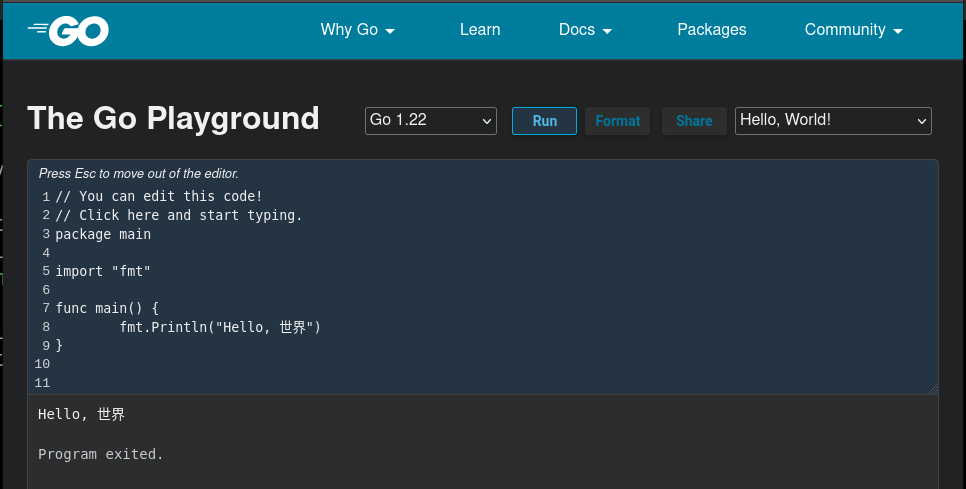
\includegraphics[width=\textwidth]{playground}
	\end{center}
\end{frame}
\begin{frame}[fragile]{Importing Third-Party Packages}
	\begin{itemize}
		\item Standard library package names are simple names:
			\begin{lstlisting}
import "fmt"
import "encoding/json"
import "flag"
import "math"
\end{lstlisting}
\pause
		\item Getting packages from public repositories:
\begin{lstlisting}
import "github.com/MadScienceZone/go-gma/v5/dice"
\end{lstlisting}
	\end{itemize}
	\vfill
	\strut
\end{frame}
\begin{frame}{Automatic API Documentation}
\begin{itemize}
\item\z{https://pkg.go.dev/}\emph{repository-url}
\end{itemize}
	\begin{center}
		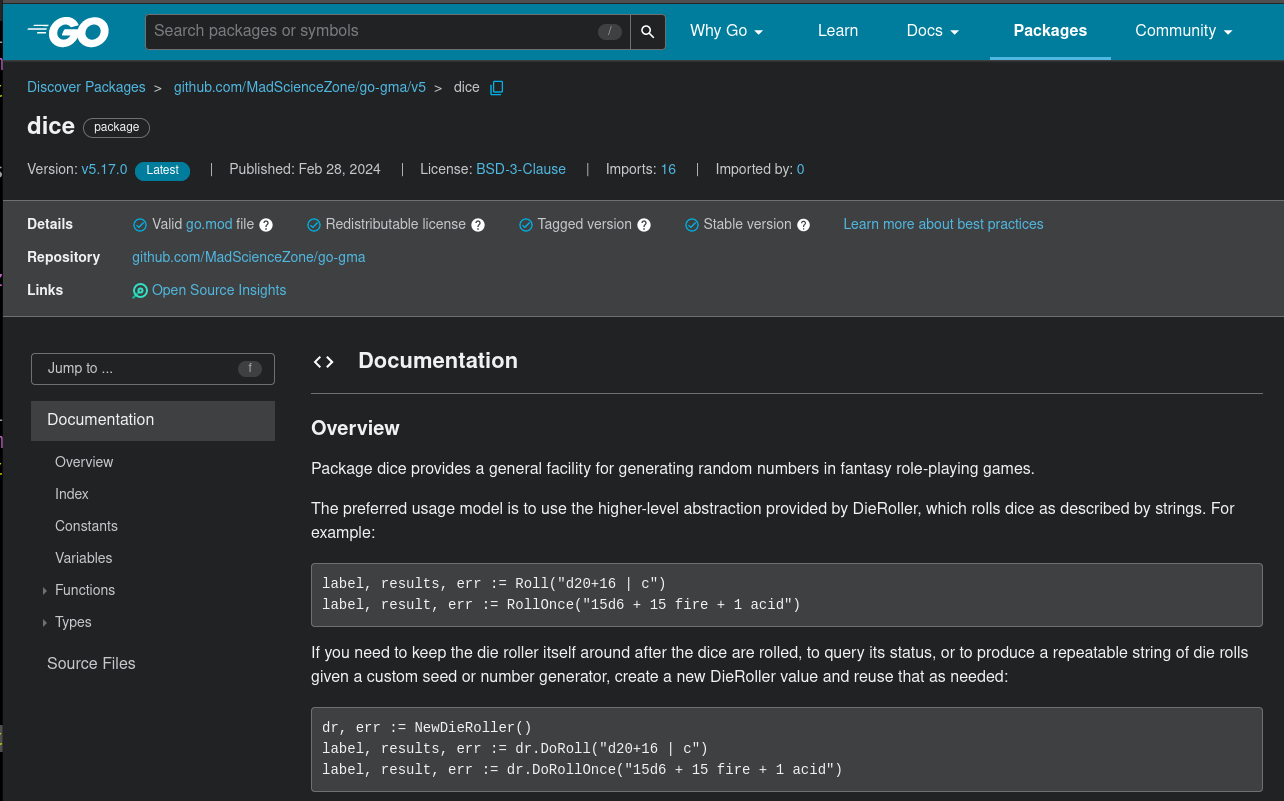
\includegraphics[width=\textwidth]{docsite}
	\end{center}
\end{frame}

\begin{frame}[fragile]{``Factored'' Notation}
\begin{lstlisting}
import "fmt"
import "encoding/json"
import "flag"
import "math"
\end{lstlisting}
\pause
\begin{lstlisting}
import (
   "fmt"
   "encoding/json"
   "flag"
   "math"
)
\end{lstlisting}
\end{frame}

\begin{frame}[fragile]{``Factored'' Notation}
\begin{lstlisting}
var initialized bool
var userNames   []string
var Greeting    string   = "Hello"
var TheAnswer            = 42
\end{lstlisting}
\begin{lstlisting}
var (
    initialized bool
    userNames   []string
    Greeting    string   = "Hello"
    TheAnswer            = 42
)
\end{lstlisting}
\end{frame}

\begin{frame}[fragile]{``Factored'' Notation}
\begin{lstlisting}
const initialized = false
const Greeting    = "Hello"
const TheAnswer   byte = 42
\end{lstlisting}
\begin{lstlisting}
const (
    initialized      = false
    Greeting         = "Hello"
    TheAnswer   byte = 42
)
\end{lstlisting}
\end{frame}

\begin{frame}[fragile]{``Factored'' Notation and iota}
\begin{onlyenv}<1->
\begin{lstlisting}
type MessageType byte
const (
    ServerCommand MessageType = 0
    ServerReply   MessageType = 1
    ServerError   MessageType = 2
    UrgentMessage MessageType = 3
)
\end{lstlisting}
\end{onlyenv}
\vfill\strut
\begin{onlyenv}<2>
\begin{lstlisting}
type MessageType byte
const (
    ServerCommand MessageType = iota
    ServerReply   MessageType = iota
    ServerError   MessageType = iota
    UrgentMessage MessageType = iota
)
\end{lstlisting}
\end{onlyenv}
\begin{onlyenv}<3>
\begin{lstlisting}
type MessageType byte
const (
    ServerCommand MessageType = iota
    ServerReply   
    ServerError   
    UrgentMessage 
)
\end{lstlisting}
\end{onlyenv}
\end{frame}
\begin{frame}[fragile]{``Factored'' Notation and iota Expressions}
\begin{lstlisting}
type MessageType byte
const (
    ServerCommand MessageType = 0x01
    ServerReply   MessageType = 0x02
    ServerError   MessageType = 0x04
    UrgentMessage MessageType = 0x08
)
\end{lstlisting}
\vfill\strut
\begin{lstlisting}
type MessageType byte
const (
    ServerCommand MessageType = 1 << iota
    ServerReply   
    ServerError   
    UrgentMessage 
)
\end{lstlisting}
\end{frame}

\subsubsection{Collection Types}
\begin{frame}[fragile]{Arrays}
	\begin{itemize}
		\item No, never mind. Let's talk about slices instead.
	\end{itemize}
\end{frame}

\begin{frame}[fragile]{Slices}
\begin{lstlisting}
var Ages map[string]int
Ages = make(map[string]int, 10)

Ages["Alice"] = 14
Ages["Bob"] = 22
Ages["Charlie"] = 27
Ages["Daria"] = 42
fmt.Println(Ages)

for name, age := range Ages {
    if age >= 18 {
        fmt.Printf("%s is allowed to vote.\n", name)
    } else {
        fmt.Printf("%s is not eligible to vote.\n", name)
    }
}
\end{lstlisting}
\end{frame}
\begin{frame}[fragile]{Maps}
\end{frame}
\subsubsection{Control Flow}
\begin{frame}[fragile]{Conditionals}
% if for switch 
\end{frame}
\begin{frame}[fragile]{Loops}
\end{frame}

\subsection{Object Oriented Features}
\begin{frame}[fragile]{Structures}
\end{frame}

\begin{frame}[fragile]{Method Functions}
\end{frame}

\begin{frame}[fragile]{Composition}
\end{frame}

\begin{frame}[fragile]{Polymorphism}
\end{frame}

\section[Concurrency]{Concurrency}
\subsection{Goroutines}

\begin{frame}[fragile]{Goroutines---Calling a Function in the ``Background''}
\begin{lstlisting}
func countdown() {
    for i := 10; i >= 0; i-- {
        fmt.Printf(">>> %d <<<\n", i)
        time.Sleep(1 * time.Second)
    }
}
\end{lstlisting}
\pause
\begin{lstlisting}
func main() {
    countdown()
    fmt.Println("Starting a long-running task...")
    time.Sleep(15 * time.Second)
    fmt.Println("Done. Exiting.")
}
\end{lstlisting}
\end{frame}

\begin{frame}[fragile]{Goroutines---Calling a Function in the ``Background''}
\begin{lstlisting}
func countdown() {
    for i := 10; i >= 0; i-- {
        fmt.Printf(">>> %d <<<\n", i)
        time.Sleep(1 * time.Second)
    }
}
\end{lstlisting}
\begin{lstlisting}
func main() {
    go countdown()
    fmt.Println("Starting a long-running task...")
    time.Sleep(15 * time.Second)
    fmt.Println("Done. Exiting.")
}
\end{lstlisting}
\end{frame}




\subsection{Thread-Safe Memory Access}
\begin{frame}[fragile]{Global ID Generation (Na\"\i ve)}
\begin{lstlisting}
type GameState struct {
    NextMessageID int
}
\end{lstlisting}
\pause
\begin{lstlisting}
var gameServer GameState

gameServer.NextMessageID++
client.ID = gameServer.NextMessageID
\end{lstlisting}
\end{frame}

\begin{frame}[fragile]{Global ID Generation (Mutex)}
\begin{onlyenv}<1>
\begin{lstlisting}
type GameState struct {
    NextMessageID int
    Lock          sync.Mutex
}
\end{lstlisting}
\end{onlyenv}
\begin{onlyenv}<2->
\begin{lstlisting}
type GameState struct {
    NextMessageID int
    Lock          sync.RWMutex
}
\end{lstlisting}
\end{onlyenv}
\begin{onlyenv}<3-4>
\begin{lstlisting}
func (state *GameState) GetNextID() int {
    state.Lock.Lock()
    state.NextMessageID++
    nextID := state.MessageID
    state.Lock.Unlock()
    return nextID
}
\end{lstlisting}
\end{onlyenv}
\begin{onlyenv}<5>
\begin{lstlisting}
func (state *GameState) GetNextID() int {
    state.Lock.Lock()
    defer state.Lock.Unlock()

    state.NextMessageID++
    return state.NextMessageID
}
\end{lstlisting}
\end{onlyenv}
\begin{onlyenv}<4->
\begin{lstlisting}
client.ID = gameServer.GetNextID()
\end{lstlisting}
\end{onlyenv}
\end{frame}

\begin{frame}[fragile]{Global ID Generation (Channel)}
\begin{lstlisting}
func serveMessageIDs(c chan int) int {
    var id int
    for {
        c <- id
        c++
    }
}
\end{lstlisting}
\pause
\begin{lstlisting}
IDSource := make(chan int)
go serveMessageIDs(IDSource)
\end{lstlisting}
\pause
\begin{lstlisting}
client.ID = <-IDSource
\end{lstlisting}
\end{frame}

\begin{frame}[fragile]{Channels}
\begin{lstlisting}
ch := make(chan byte)
\end{lstlisting}
\pause
\begin{lstlisting}
fmt.Println("Writing to channel")
\end{lstlisting}
\identifier{ch}\z{ <- 42}
\pause
\begin{lstlisting}
fmt.Println("Reading from channel")
x := <-ch
fmt.Println("Read", x, "from channel")
\end{lstlisting}
\end{frame}

\begin{frame}[fragile]{Channels}
\begin{lstlisting}
ch := make(chan byte)
\end{lstlisting}
\begin{lstlisting}
fmt.Println("Writing to channel")
\end{lstlisting}
{\color{red}\z{ch <- 42\qquad\qquad// DEADLOCKED!}}
\begin{lstlisting}
fmt.Println("Reading from channel")
x := <-ch
fmt.Println("Read", x, "from channel")
\end{lstlisting}
\end{frame}

\begin{frame}[fragile]{Channels}
\begin{lstlisting}
ch := make(chan byte)
go func(c chan byte) {
    x := <-c
    fmt.Println("Read", x, "from channel")
}(ch)

fmt.Println("Writing to channel")
ch <- 42
\end{lstlisting}
\end{frame}

\begin{frame}[fragile]{Buffered Channels}
\begin{lstlisting}
\end{lstlisting}
ch := make(chan byte, 1)
\pause
\begin{lstlisting}
fmt.Println("Writing to channel")
ch <- 42

fmt.Println("Reading from channel")
x := <-ch
fmt.Println("Read", x, "from channel")
\end{lstlisting}
\end{frame}

\subsection{}
% interface any
% select

%
% backup
% type assertions/switch
% contexts
\end{document}
